\section{Vertices}
%<-------------------------------------------------------------------------->
\tkzcname{Vertex} is the main macro: it places a vertex. A vertex can be
placed with cartesian or polar coordinates, on an existing node, or relatively
to another vertex.

\subsection{\tkzcname{Vertex}}
\begin{NewMacroBox}{Vertex}{\oarg{local options}\var{name}}
A vertex has a name, a position, a label and a style.

\medskip
The argument \IargName{Vertex}{name} is mandatory: it is the name of the
\TIKZ\ node, used later to draw the edges. Do not confuse it with the
\tkzname{label}, the text displayed in the vertex: the name can be
\tkzname{M1} and the label $M_1$.

\medskip
\begin{tabular}{llc}
\toprule
Options   & Default  & Definition              \\
\midrule
\TOline{x}        {\{\}}{abscissa}
\TOline{y}        {\{\}}{ordinate}
\TOline{a}        {\{\}}{angle (polar coordinates)}
\TOline{d}        {\{\}}{distance (polar coordinates)}
\TOline{Node}     {false}{the vertex is placed on an existing node}
\TOline{position} {\{\}}{\TIKZ\ relative placement (\tkzname{right=of A}\dots)}
\TOline{unit}     {\textbackslash GraphUnit}{distance for the shortcuts}
\TOline{dir}      {\textbackslash EA}{direction used by \tkzcname{Vertices}}
\TOline{style}    {\{\}}{\TIKZ\ options added to the node}
\midrule
\TOline{empty}    {false}{the vertex is an invisible node}
\midrule
\TOline{NoLabel}  {false}{no label}
\TOline{LabelOut} {false}{the label is outside the node}
\TOline{L}        {\{\}}{the label}
\TOline{Math}     {false}{the label is written in math mode}
\TOline{Ldist}    {0cm}{distance between the node and an outside label}
\TOline{Lpos}     {0}{angle of an outside label}
\bottomrule
\end{tabular}

\medskip
\emph{If \tkzname{L} is empty, the label is the name of the vertex.
Without \tkzname{x}, \tkzname{y}, \tkzname{a}, \tkzname{d} and
\tkzname{position}, the vertex is placed at the origin.}
\end{NewMacroBox}

\subsubsection{Cartesian coordinates}
\tkzcname{Vertex}\tkzname{[x=\meta{number},y=\meta{number}]}\var{name}.

\begin{tkzexample}[latex=7cm,small]
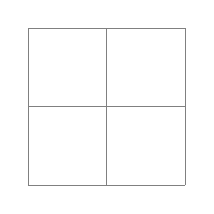
\begin{tikzpicture}
  \draw[help lines] (0,0) grid (2,2);
  \Vertex{A} % x=0, y=0
  \Vertex[x=2,y=0]{B}
  \Vertex[x=2,y=2]{C}
\end{tikzpicture}
\end{tkzexample}

\subsubsection{Polar coordinates}
\tkzcname{Vertex}\tkzname{[a=\meta{angle},d=\meta{distance}]}\var{name}.

\begin{tkzexample}[latex=7cm,small]
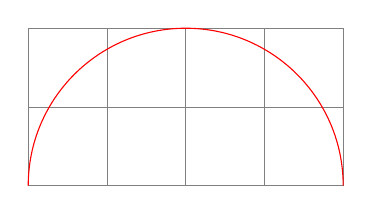
\begin{tikzpicture}
  \draw[help lines] (-2,0) grid (2,2);
  \draw[red] (2,0) arc (0:180:2cm);
  \Vertex{A}
  \Vertex[a=45,d=2cm]{B}
  \Vertex[a=135,d=2cm]{C}
\end{tikzpicture}
\end{tkzexample}

\subsubsection{Option \tkzname{Node}: a vertex on an existing node}
The vertex is placed on a node or on a \tkzname{coordinate} already defined.

\begin{tkzexample}[latex=7cm,small]
\begin{tikzpicture}
  \draw[help lines] (0,0) grid (2,2);
  \Vertex{A} \Vertex[x=2,y=2]{B}
  \coordinate (M) at ($(A)!.5!(B)$);
  \Vertex[Node]{M}
\end{tikzpicture}
\end{tkzexample}

\subsubsection{Option \tkzname{position}: placement with \TIKZ}
With the library \tkzname{positioning}:

\begin{tkzexample}[latex=7cm,small]
\begin{tikzpicture}[node distance=2cm]
  \Vertex{A}
  \Vertex[position={right=of A}]{B}
  \Vertex[position={above right=of A}]{C}
  \Edges(A,B,C,A)
\end{tikzpicture}
\end{tkzexample}

\subsubsection{Option \tkzname{empty}: an invisible vertex}
The node exists (edges can reach it) but nothing is drawn.

\begin{tkzexample}[latex=7cm,small]
\begin{tikzpicture}
  \Vertex{A}
  \Vertex[x=3,y=0,empty]{B}
  \Edge(A)(B)
\end{tikzpicture}
\end{tkzexample}

\newpage
%<-------------------------------------------------------------------------->
\subsection{Relative placement: the shortcuts}
%<-------------------------------------------------------------------------->
A distance between two vertices is needed: the unit of the graph.

\begin{NewMacroBox}{SetGraphUnit}{\var{number}}
\emph{Sets the distance between the centers of two vertices placed with a
shortcut. The number is expressed in the units of \TIKZ\ (1 cm by default).
The default value is $1$. The definition is local to a group or a
\tkzname{scope} environment.}
\end{NewMacroBox}

\begin{NewMacroBox}{EA}{\oarg{local options}\varp{vertex A}\var{vertex B}}
\emph{The shortcuts create \tkzname{vertex B} relatively to
\tkzname{vertex A}. The distance is \tkzname{unit} horizontally and
vertically: \tkzname{unit} is given by \tkzcname{SetGraphUnit} (or by
\tkzcname{GraphInit}, or \tkzcname{tkzSetUpGraph}) or by the option
\tkzname{unit}. The options are those of \tkzcname{Vertex}.}

\medskip
\begin{tabular}{ll}
\toprule
Shortcut   & Definition              \\
\midrule
\tkzcname{EA}   & east \\
\tkzcname{WE}   & west \\
\tkzcname{NO}   & north \\
\tkzcname{SO}   & south \\
\tkzcname{NOEA} & north-east (north then east) \\
\tkzcname{NOWE} & north-west \\
\tkzcname{SOEA} & south-east \\
\tkzcname{SOWE} & south-west \\
\bottomrule
\end{tabular}

\medskip
\emph{With \tkzcname{NOEA}, the distance between the two vertices is
$\sqrt{2}\times$\tkzname{unit}.}
\end{NewMacroBox}

\subsubsection{The shortcuts with the default unit}
\begin{tkzexample}[latex=7cm,small]
\begin{tikzpicture}
  \draw[help lines] (-1,-1) grid (1,1);
  \Vertex{A}
  \EA(A){B}   \WE(A){C}   \NO(A){D}   \SO(A){E}
  \NOEA(A){F} \NOWE(A){G} \SOEA(A){H} \SOWE(A){I}
  \foreach \v in {B,C,D,E,F,G,H,I}{\Edge(A)(\v)}
\end{tikzpicture}
\end{tkzexample}

\subsubsection{A new unit with \tkzcname{SetGraphUnit}}
\begin{tkzexample}[latex=7cm,small]
\begin{tikzpicture}
  \draw[help lines] (-2,-2) grid (2,2);
  \SetGraphUnit{2}
  \Vertex{A}
  \EA(A){B}   \WE(A){C}   \NO(A){D}   \SO(A){E}
  \NOEA(A){F} \NOWE(A){G} \SOEA(A){H} \SOWE(A){I}
  \foreach \v in {B,C,D,E,F,G,H,I}{\Edge(A)(\v)}
\end{tikzpicture}
\end{tkzexample}

\subsubsection{The units of \TIKZ: \tkzname{x=2cm,y=1cm}}
\begin{tkzexample}[latex=7cm,small]
\begin{tikzpicture}[x=2cm,y=1cm]
  \draw[help lines] (-1,-1) grid (1,1);
  \Vertex{A}
  \EA(A){B}   \WE(A){C}   \NO(A){D}   \SO(A){E}
  \NOEA(A){F} \NOWE(A){G} \SOEA(A){H} \SOWE(A){I}
  \foreach \v in {B,C,D,E,F,G,H,I}{\Edge(A)(\v)}
\end{tikzpicture}
\end{tkzexample}

\subsubsection{A graph built from a coordinate}
\begin{tkzexample}[latex=7cm,small]
\begin{tikzpicture}
  \draw[help lines] (-2,-2) grid (4,2);
  \SetGraphUnit{2}
  \coordinate (O) at (0,0);
  \NOEA(O){A} \NOWE(O){B} \SOEA(O){D}
  \SOWE(O){C} \NOEA(D){E}
  \Edges(B,C,D,A,E,D,B,A,C)
\end{tikzpicture}
\end{tkzexample}

\subsubsection{A local unit}
The option \tkzname{unit}, a \tkzname{scope} environment or a \TEX\ group
limit the change of unit.

\begin{tkzexample}[latex=7cm,small]
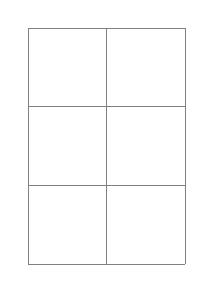
\begin{tikzpicture}
  \draw[help lines] (0,0) grid (2,3);
  \SetGraphUnit{2}
  \Vertex{A}  \EA(A){B}
  \NO[unit=3](B){C}
  {\SetGraphUnit{1} \NO(A){D}}
  \NO(D){E}
\end{tikzpicture}
\end{tkzexample}

\endinput
